
\documentclass[aspectratio=1610]{beamer}
\usetheme{boxes}
\usecolortheme{crane}
\usepackage{amsmath,amsfonts}
\usepackage{algpseudocode}
\usepackage{multicol}
\usepackage{pgfplots}
\pgfplotsset{compat=1.15}
\usepackage{mathrsfs}
\usetikzlibrary{arrows}


%-------------------------------------------------------------------
%	 TITLE SLIDE
%-------------------------------------------------------------------

\title{\huge{Programming is not Coding}}
\subtitle{How to build safe and secure software}
\author{Stefan Parvu}

%\titlegraphic{\includegraphics[scale=0.25]{Images/bugs.pdf}} 
% Optional title page image, comment this line to remove it

%\institute{Institute Name \\ Institute Address}

%\date{dd mm yyyy}
%\setlength{\columnsep}{90pt}


\begin{document}

\begin{frame}[plain,noframenumbering]
\makebox[\linewidth]{
\includegraphics[width=\paperwidth]{Images/Intro-CS.png}}
\end{frame}


\begin{frame}
	\maketitle % Automatically created using the information in the commands
\end{frame}

%\begin{frame}
%\frametitle{Table of Contents}
%\tableofcontents[hideallsubsections]
%\tableofcontents[hideallsubsections,currentsection]
%\end{frame}


\begin{frame}
\frametitle{Table of Contents}
%\Large{Introduction to Computer Science}\\~\\
\tableofcontents

%    \begin{columns}[onlytextwidth,T]
%     
%        \begin{column}{.50\textwidth}
%            \vfill
%            \tableofcontents[sections=1-4]
%        \end{column}
% 
%        \begin{column}{.45\textwidth}
%        		\vfill
%            \tableofcontents[sections=5-7]
%        \end{column}
% 
%    \end{columns}
\end{frame}



% -------------------------------------------------------------------
% Lesson 1
% -------------------------------------------------------------------
\section{Computation. Algorithms. Programs}

\begin{frame}
\begin{center}
\Huge Lesson 1\\~\\
\textbf{Computation. Algorithms. Computer Programs}
\end{center}
\end{frame}


\begin{frame}
\frametitle{Lesson 1}

\Huge In this lesson we will talk about the following concepts:
 \alert{computation},
 \alert{algorithms} and
 \alert{programs}. 

\end{frame}


\begin{frame}{Lesson 1}{}
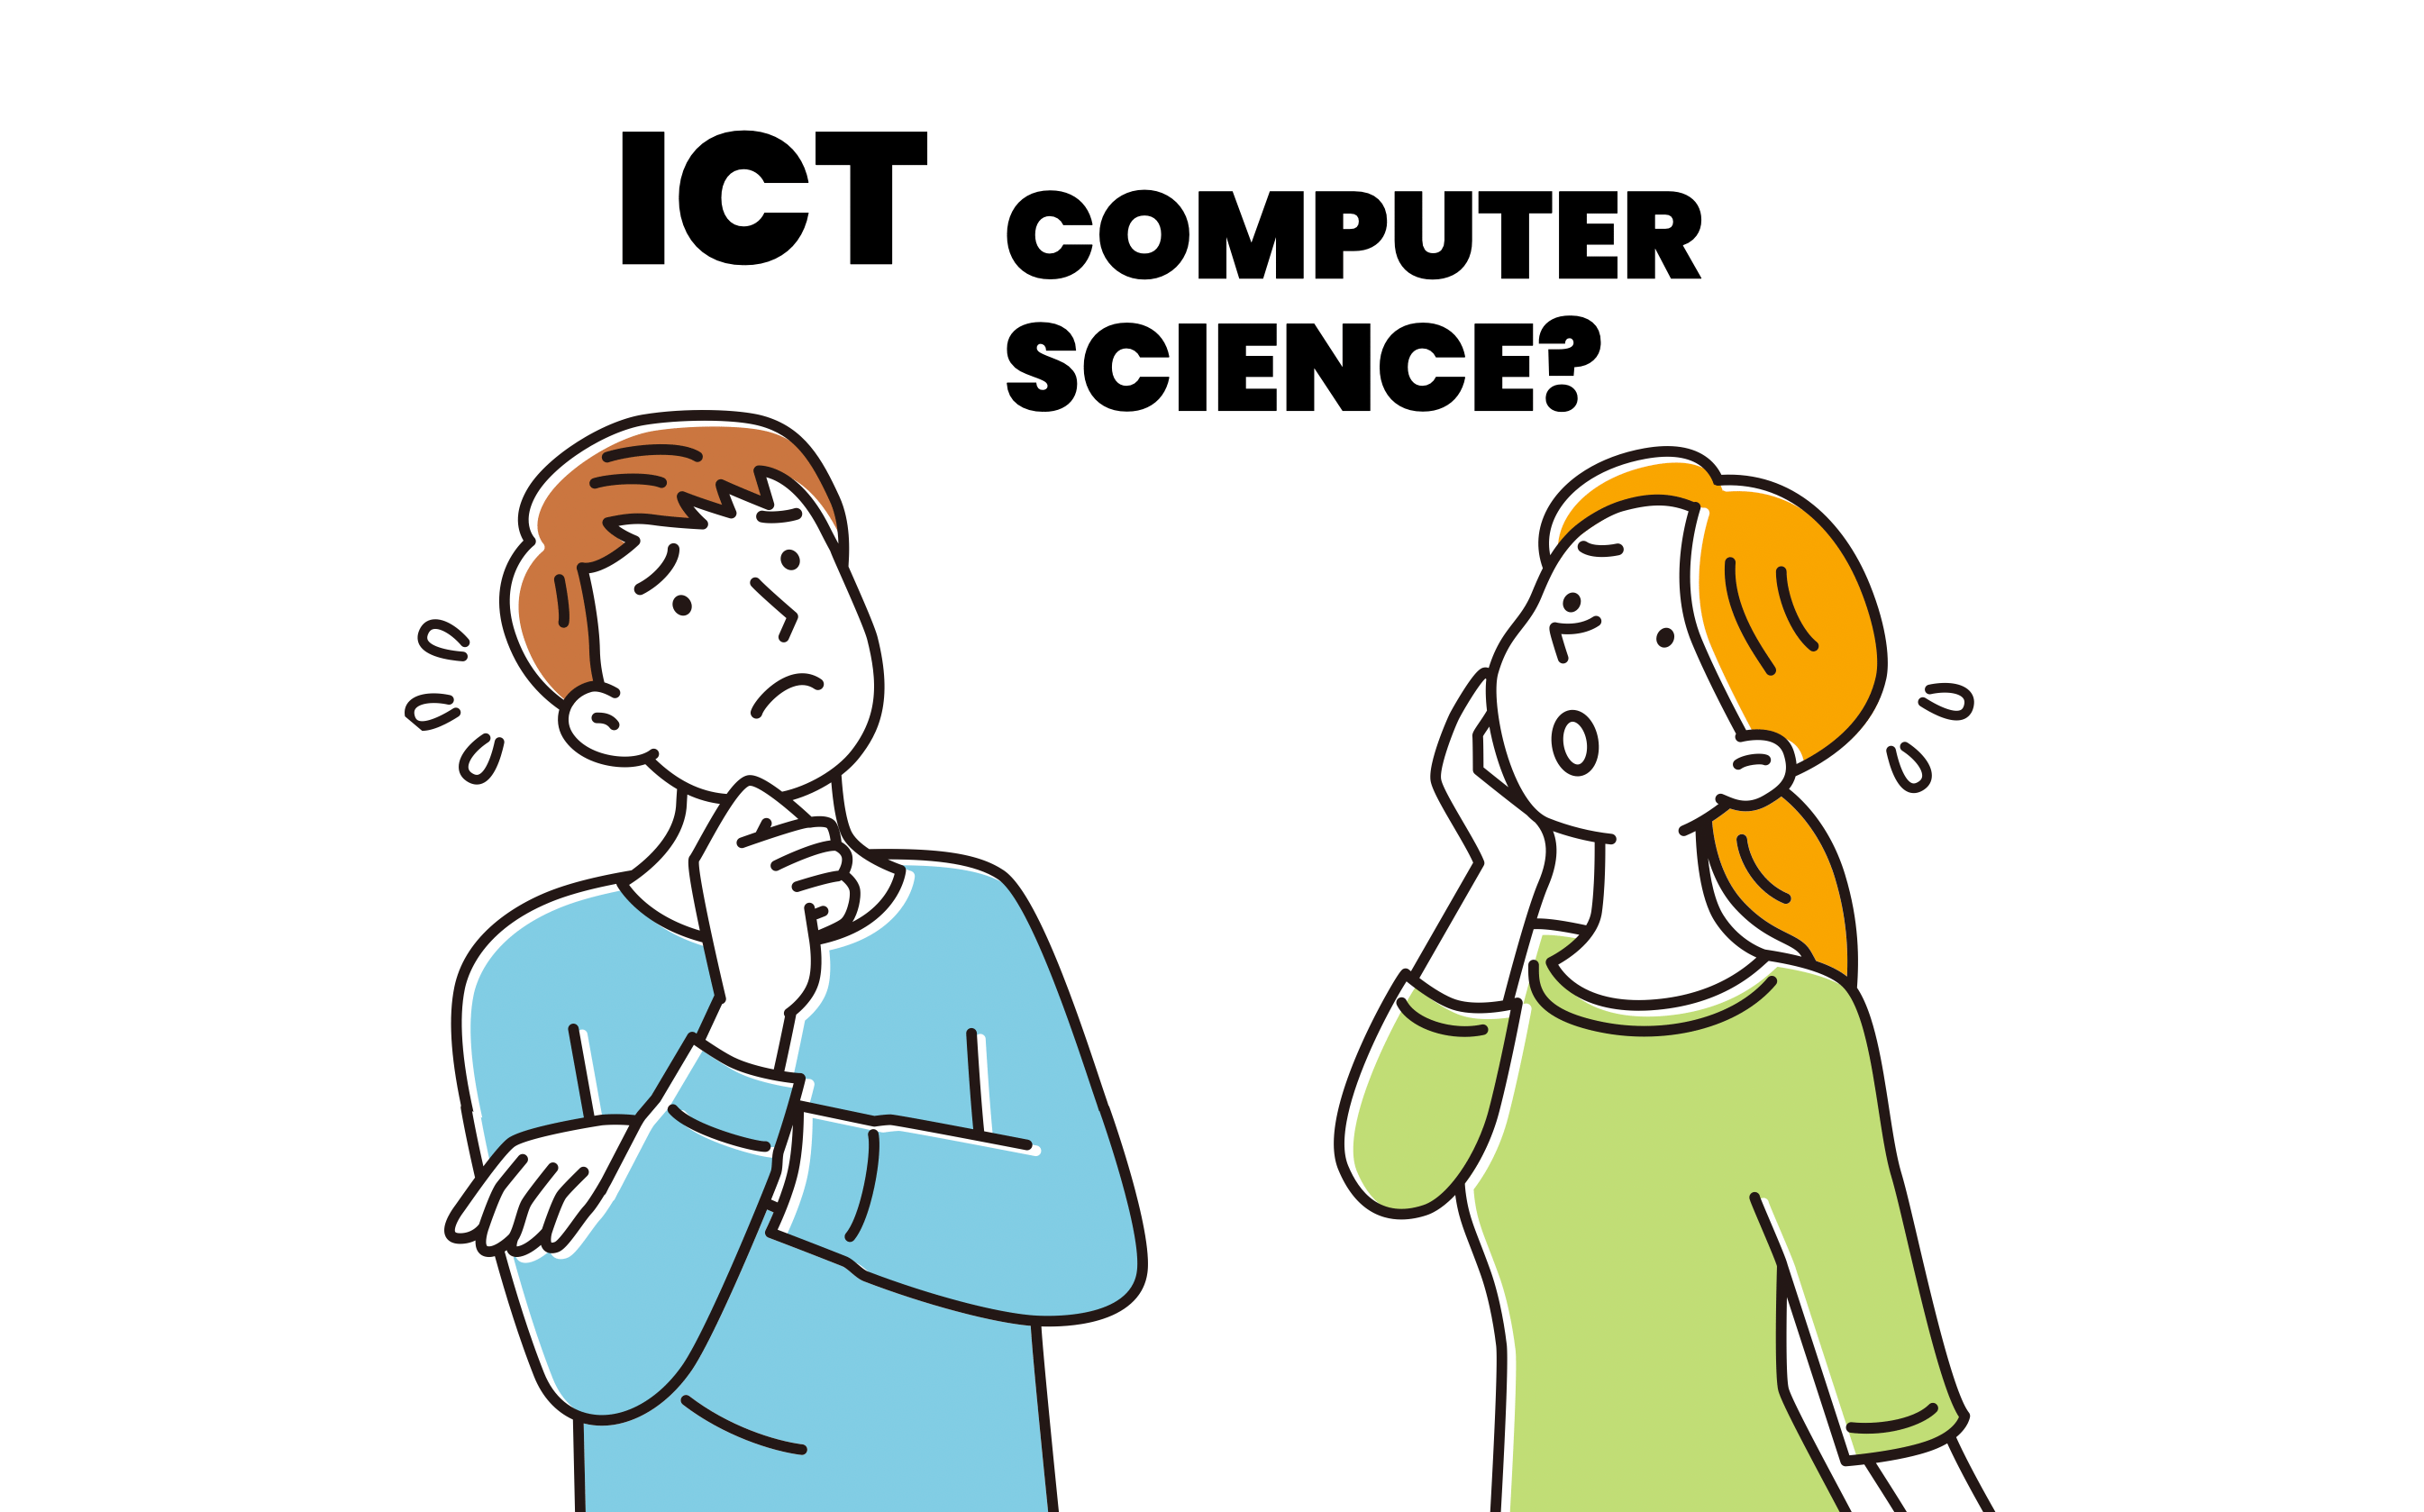
\includegraphics[scale=0.149]{Images/ictvscs.png}
\end{frame}


\begin{frame}
\begin{center}
\Huge Computer Science (CS)\\~\\
\textbf { But what's the difference between IT and CS? }
\end{center}
\end{frame}


\begin{frame}{Lesson 1}{}
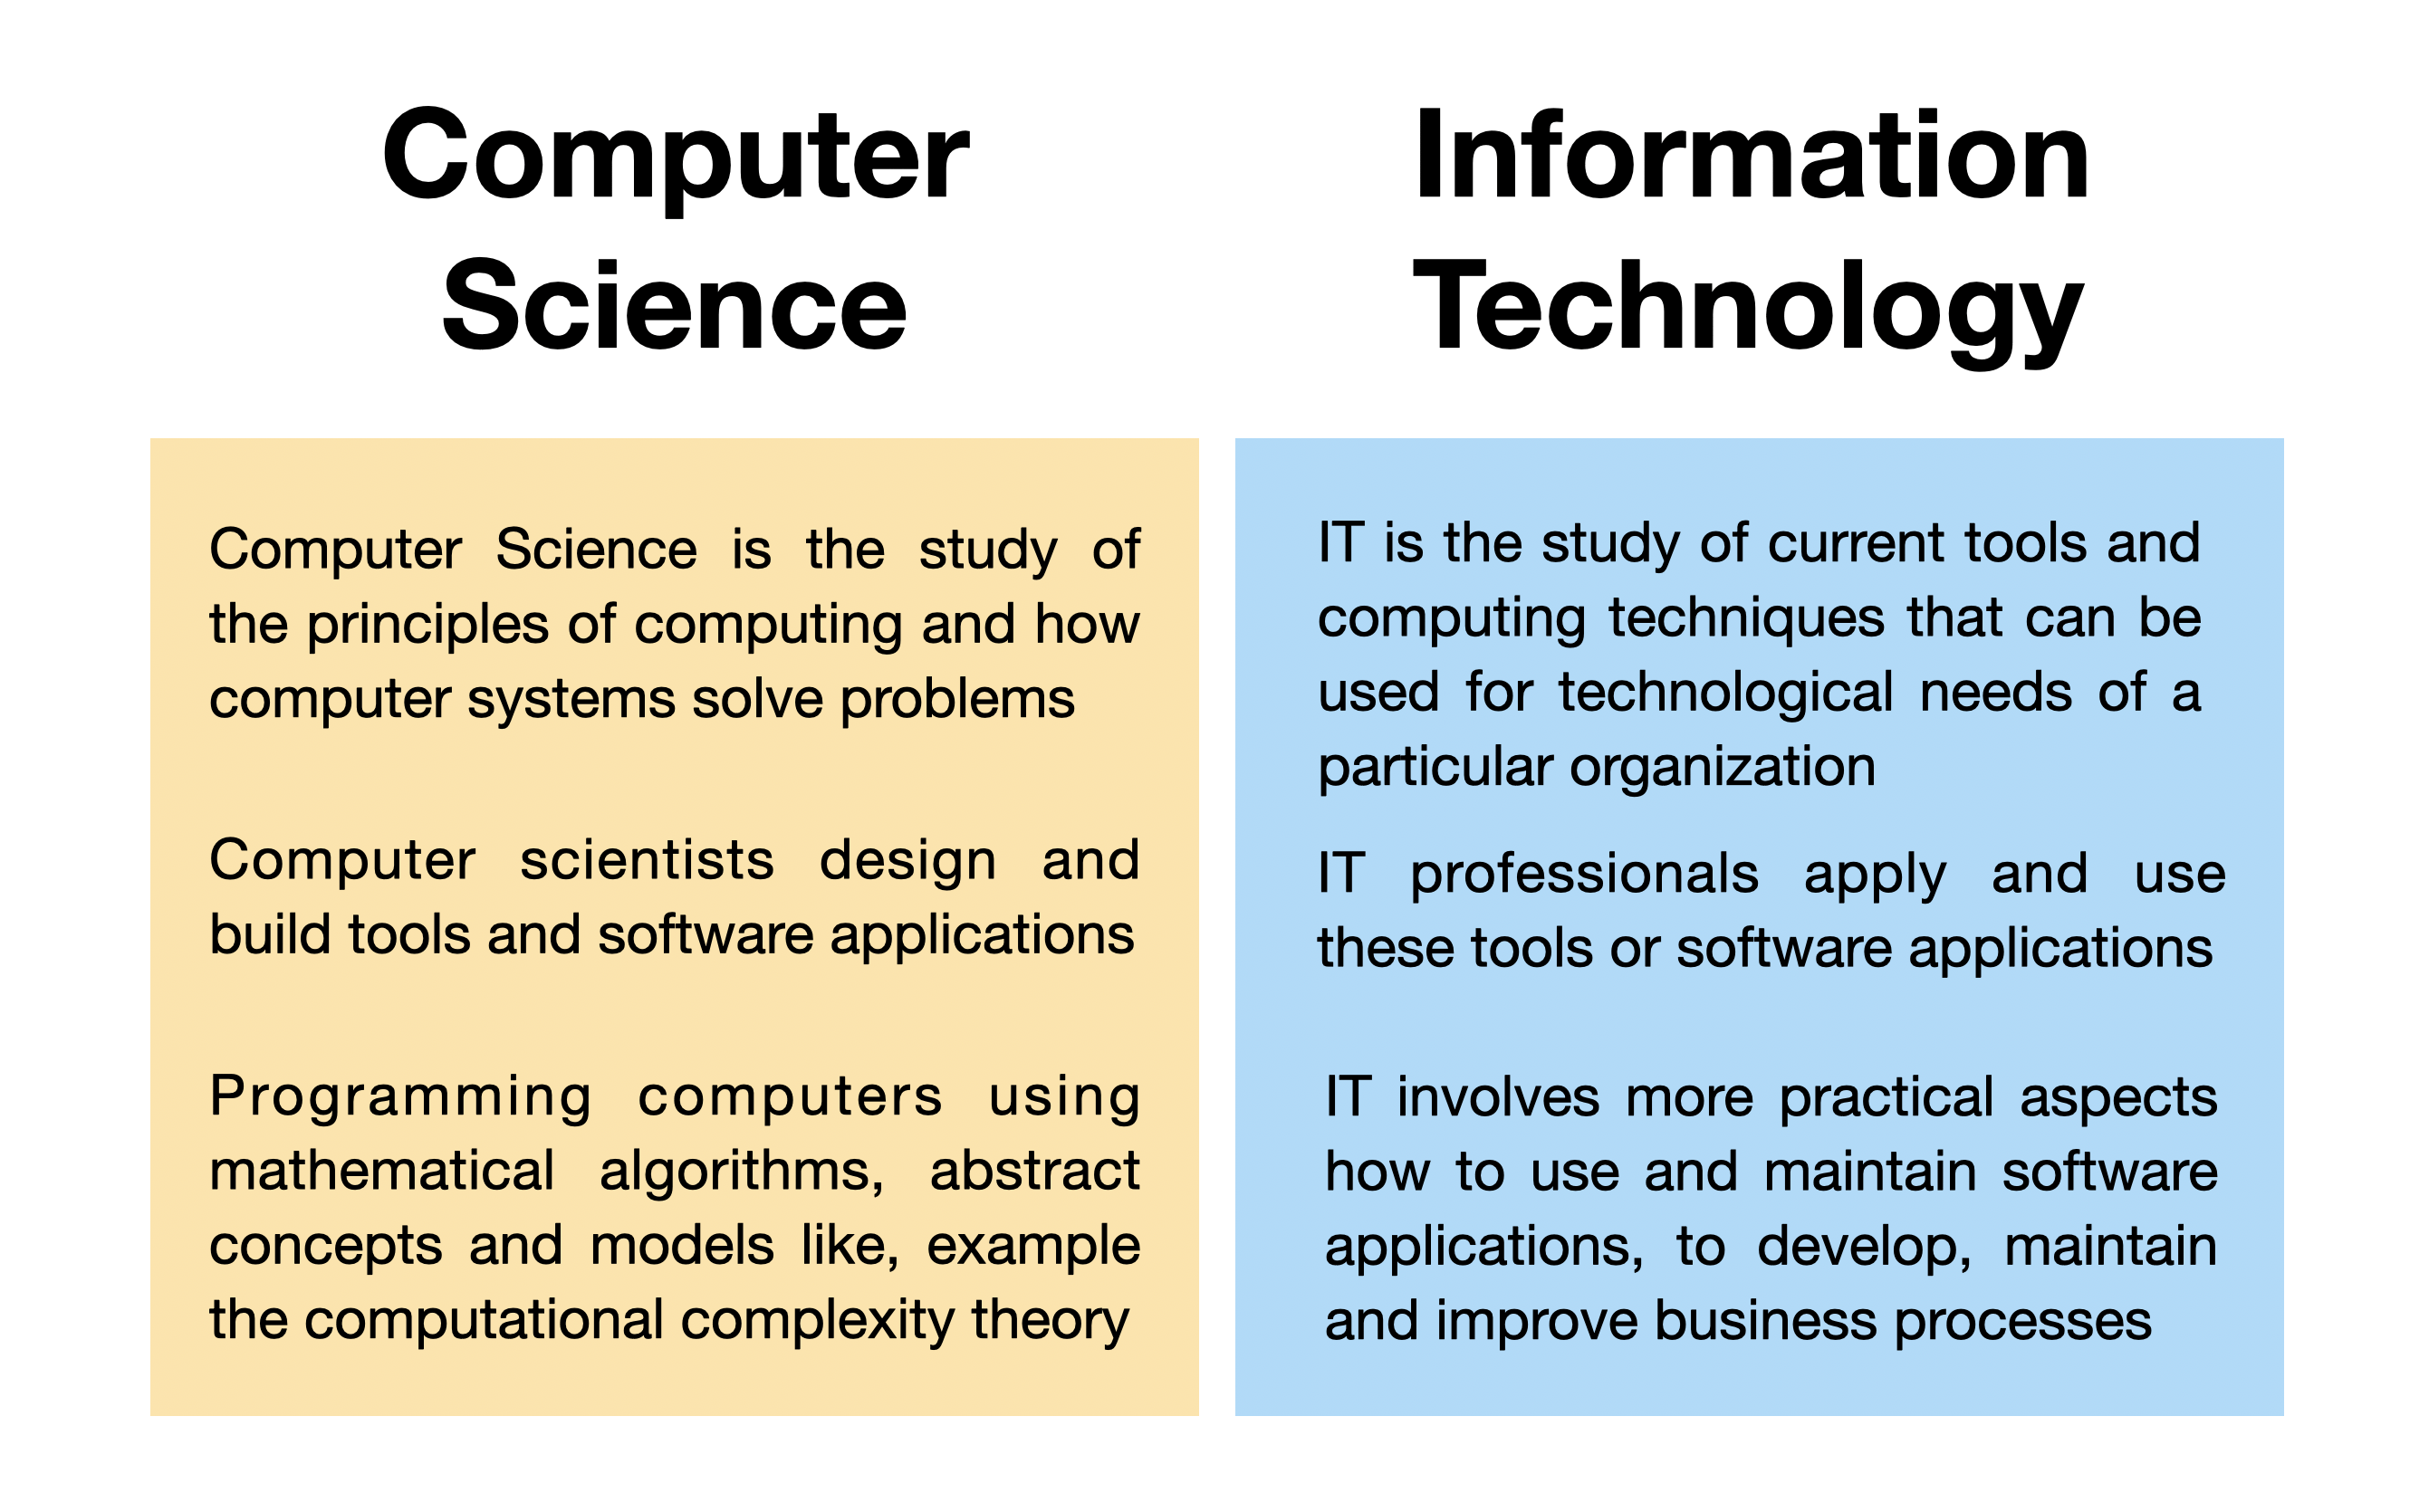
\includegraphics[scale=0.15]{Images/csvsit.png}
\end{frame}

\begin{frame}{Lesson 1}{}
\begin{center}
\Huge \textbf{Computation}
\end{center}
\end{frame}

\begin{frame}{Lesson 1}{}
{\Huge{What is a Computation?}}
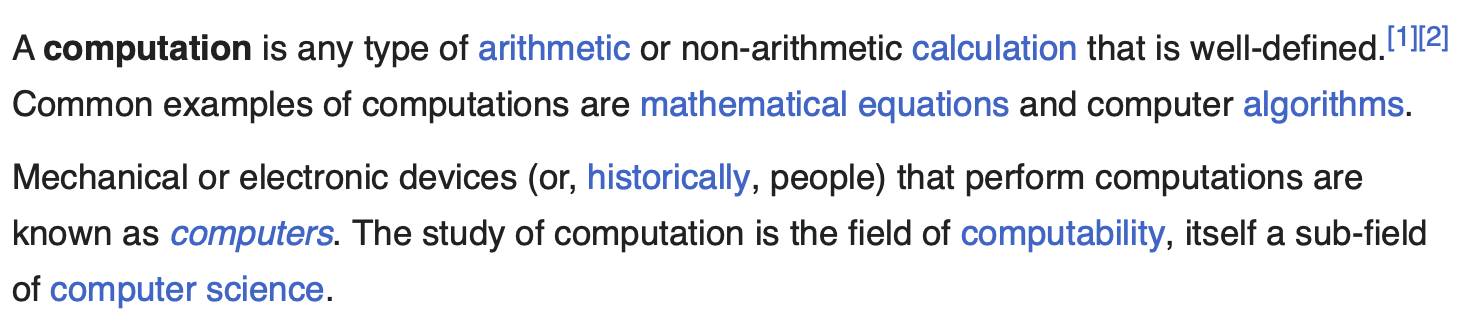
\includegraphics[scale=0.58]{Images/computation.png}
\end{frame}



\begin{frame}{Lesson 1}{}
\Huge
A \textbf{computation} is what a \alert{computing device} does\\~\\

\Large
We sometimes call the computation, a behaviour

\end{frame}



\begin{frame}{Lesson 1}{}
\LARGE
\textbf{Computing device}\\~\\
\Large
For example, a computer system, a tablet, a mobile phone or a basic calculator. But it can be as well, a non physical device, something more abstract, like an \alert{algorithm}.\\~\\

We describe a computing device by describing all its possible computations or its behaviours. 

\end{frame}



\begin{frame}{Lesson 1}{}
\LARGE
\textbf{But what is an algorithm?}\\~\\


\begin{center}

\tikzset{every picture/.style={line width=0.75pt}} %set default line width to 0.75pt        

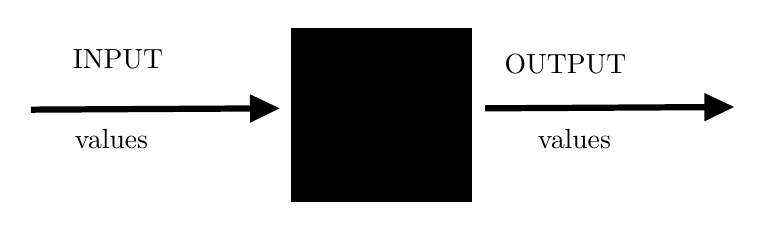
\begin{tikzpicture}[x=0.75pt,y=0.75pt,yscale=-1,xscale=1]
%uncomment if require: \path (0,171); %set diagram left start at 0, and has height of 171

%Shape: Rectangle [id:dp3842912892539916] 
\draw  [fill={rgb, 255:red, 0; green, 0; blue, 0 }  ,fill opacity=1 ][line width=2.25]  (349,57) -- (433,57) -- (433,138) -- (349,138) -- cycle ;
%Straight Lines [id:da6734653265949071] 
\draw [line width=2.25]    (440.9,94.36) -- (555.8,93.74) ;
\draw [shift={(560.8,93.71)}, rotate = 179.69] [fill={rgb, 255:red, 0; green, 0; blue, 0 }  ][line width=0.08]  [draw opacity=0] (14.29,-6.86) -- (0,0) -- (14.29,6.86) -- cycle    ;
%Straight Lines [id:da6306489033059055] 
\draw [line width=2.25]    (222,95) -- (336.9,94.38) ;
\draw [shift={(341.9,94.36)}, rotate = 179.69] [fill={rgb, 255:red, 0; green, 0; blue, 0 }  ][line width=0.08]  [draw opacity=0] (14.29,-6.86) -- (0,0) -- (14.29,6.86) -- cycle    ;


% Text Node
\draw (241,65) node [anchor=north west][inner sep=0.75pt]   [align=left] {INPUT};
% Text Node
\draw (242,103) node [anchor=north west][inner sep=0.75pt]   [align=left] {values};
% Text Node
\draw (449,67) node [anchor=north west][inner sep=0.75pt]   [align=left] {OUTPUT};
% Text Node
\draw (465,103) node [anchor=north west][inner sep=0.75pt]   [align=left] {values};

\end{tikzpicture}


\end{center}

Sequence of computational steps that transform the input into the output

\end{frame}



\begin{frame}{Lesson 1}{}
\LARGE
\textbf{Example of computations}\\~\\
\begin{itemize}
    \item well-defined mathematical statements
    \item solvable statements
    \item simple instructions
\end{itemize}

\Large
\textbf{Note:} There are however other problems difficult to solve or sometimes impossible to solve because there is no algorithm for them. Like the halting problem. 
\end{frame}



\begin{frame}{Lesson 1}{}

\LARGE
\textbf{The halting problem}\\~\\
"The halting problem is the problem of determining, from a description of
an arbitrary computer program and an input, whether the program will
finish running, or continue to run forever. The halting problem is
undecidable, meaning that no general algorithm exists that solves the
halting problem for all possible program input pairs."
\end{frame}



\begin{frame}{Lesson 1}{}

\LARGE
\textbf{Computation as a Sequence of States}\\~\\

\end{frame}


\begin{frame}{Lesson 1}{}

{\LARGE\textbf{{Computation as a sequence of states}}}\\~\\

\tikzset{every picture/.style={line width=0.75pt}} %set default line width to 0.75pt        

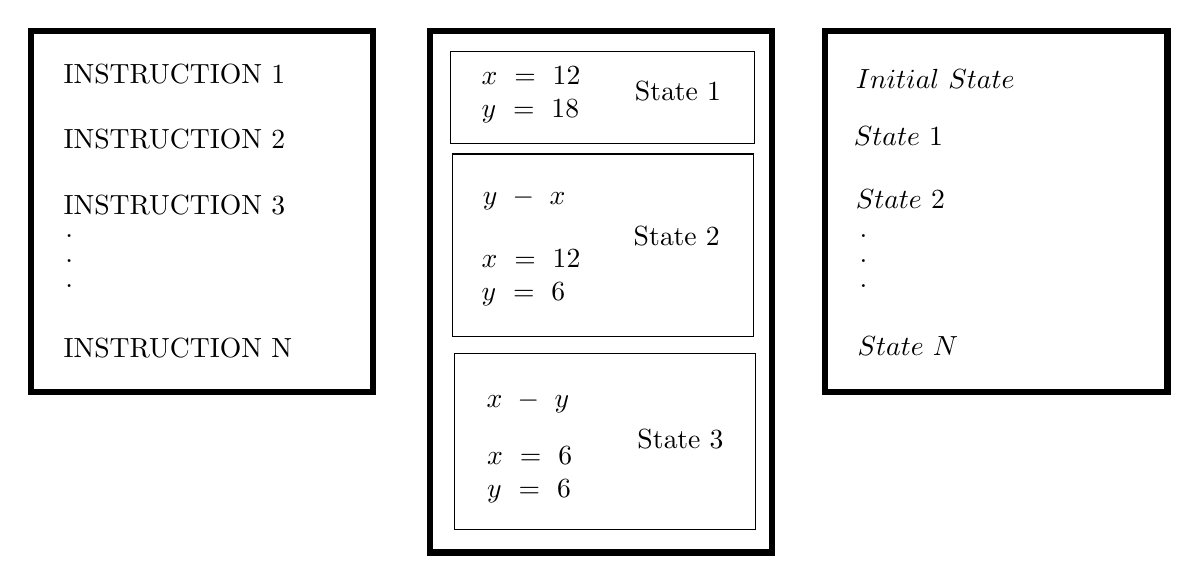
\begin{tikzpicture}[x=0.68pt,y=0.75pt,yscale=-1,xscale=1]
%uncomment if require: \path (0,274); %set diagram left start at 0, and has height of 274

%Shape: Rectangle [id:dp6019250769064086] 
\draw  [line width=2.25]  (8,8.89) -- (190.02,8.89) -- (190.02,182.89) -- (8,182.89) -- cycle ;

%Shape: Rectangle [id:dp7080615929230203] 
\draw  [line width=2.25]  (220,8.89) -- (402.02,8.89) -- (402.02,260.24) -- (220,260.24) -- cycle ;
%Shape: Rectangle [id:dp947692085619549] 
\draw   (231,19.02) -- (392.78,19.02) -- (392.78,63.25) -- (231,63.25) -- cycle ;

%Shape: Rectangle [id:dp5588602651005923] 
\draw  [line width=2.25]  (430,8.89) -- (612.02,8.89) -- (612.02,182.89) -- (430,182.89) -- cycle ;
%Shape: Rectangle [id:dp10843731413716062] 
\draw   (232,68.24) -- (392.19,68.24) -- (392.19,156.25) -- (232,156.25) -- cycle ;
%Shape: Rectangle [id:dp1566544972277042] 
\draw   (233,164.24) -- (393.19,164.24) -- (393.19,249.25) -- (233,249.25) -- cycle ;

% Text Node
\draw (24,24) node [anchor=north west][inner sep=0.75pt]   [align=left] {INSTRUCTION 1};
% Text Node
\draw (24,55) node [anchor=north west][inner sep=0.75pt]   [align=left] {INSTRUCTION 2};
% Text Node
\draw (24,87) node [anchor=north west][inner sep=0.75pt]   [align=left] {INSTRUCTION 3};
% Text Node
\draw (24,156) node [anchor=north west][inner sep=0.75pt]   [align=left] {INSTRUCTION N};
% Text Node
\draw (25,106) node [anchor=north west][inner sep=0.75pt]   [align=left] {.};
% Text Node
\draw (25,118) node [anchor=north west][inner sep=0.75pt]   [align=left] {.};
% Text Node
\draw (25,130) node [anchor=north west][inner sep=0.75pt]   [align=left] {.};
% Text Node
\draw (445,26) node [anchor=north west][inner sep=0.75pt]   [align=left] {$\displaystyle Initial\ State$};
% Text Node
\draw (445,84) node [anchor=north west][inner sep=0.75pt]   [align=left] {$\displaystyle State\ 2$};
% Text Node
\draw (447,106) node [anchor=north west][inner sep=0.75pt]   [align=left] {.};
% Text Node
\draw (447,118) node [anchor=north west][inner sep=0.75pt]   [align=left] {.};
% Text Node
\draw (447,130) node [anchor=north west][inner sep=0.75pt]   [align=left] {.};
% Text Node
\draw (446,155) node [anchor=north west][inner sep=0.75pt]   [align=left] {$\displaystyle State\ N$};
% Text Node
\draw (444,54) node [anchor=north west][inner sep=0.75pt]   [align=left] {$\displaystyle State\ 1$};
% Text Node
\draw (327.67,32.02) node [anchor=north west][inner sep=0.75pt]   [align=left] {State 1};
% Text Node
\draw (238.78,22.4) node [anchor=north west][inner sep=0.75pt]    {$ \begin{array}{l}
x\ =\ 12\ \\
y\ =\ 18
\end{array}$};
% Text Node
\draw (327,102) node [anchor=north west][inner sep=0.75pt]   [align=left] {State 2};
% Text Node
\draw (246.78,83.4) node [anchor=north west][inner sep=0.75pt]    {$y\ -\ x$};
% Text Node
\draw (248.78,181.4) node [anchor=north west][inner sep=0.75pt]    {$x\ -\ y$};
% Text Node
\draw (236,144) node [anchor=north west][inner sep=0.75pt]   [align=left] {$ $};
% Text Node
\draw (238.78,110.4) node [anchor=north west][inner sep=0.75pt]    {$ \begin{array}{l}
x\ =\ 12\ \\
y\ =\ 6
\end{array}$};
% Text Node
\draw (329,200) node [anchor=north west][inner sep=0.75pt]   [align=left] {State 3};
% Text Node
\draw (241.78,205.4) node [anchor=north west][inner sep=0.75pt]    {$ \begin{array}{l}
x\ =\ 6\ \\
y\ =\ 6
\end{array}$};


\end{tikzpicture}



\end{frame}



\begin{frame}{Lesson 1}{}

{\Large\textbf{{What is a computing state?}}}\\~\\

\Large
A state is an assignment of values to variables.



\tikzset{every picture/.style={line width=0.75pt}} %set default line width to 0.75pt        

\begin{tikzpicture}[x=0.75pt,y=0.75pt,yscale=-1,xscale=1]
%uncomment if require: \path (0,236); %set diagram left start at 0, and has height of 236

%Shape: Rectangle [id:dp9618660579176745] 
\draw   (22,126.02) -- (183.78,126.02) -- (183.78,178.04) -- (22,178.04) -- cycle ;
%Shape: Rectangle [id:dp8277264942293441] 
\draw   (214,84.24) -- (374.19,84.24) -- (374.19,178.49) -- (214,178.49) -- cycle ;
%Shape: Rectangle [id:dp20031164153050973] 
\draw   (405,87.24) -- (565.19,87.24) -- (565.19,178.49) -- (405,178.49) -- cycle ;

% Text Node
\draw (74.67,192.02) node [anchor=north west][inner sep=0.75pt]   [align=left] {State 1};
% Text Node
\draw (29.78,129.4) node [anchor=north west][inner sep=0.75pt]    {$ \begin{array}{l}
x\ =\ 12\ \\
y\ =\ 18
\end{array}$};
% Text Node
\draw (272,192) node [anchor=north west][inner sep=0.75pt]   [align=left] {State 2};
% Text Node
\draw (228.78,99.4) node [anchor=north west][inner sep=0.75pt]    {$y\ -\ x$};
% Text Node
\draw (220.78,126.4) node [anchor=north west][inner sep=0.75pt]    {$ \begin{array}{l}
x\ =\ 12\ \\
y\ =\ 6
\end{array}$};
% Text Node
\draw (420.78,104.4) node [anchor=north west][inner sep=0.75pt]    {$x\ -\ y$};
% Text Node
\draw (408,67) node [anchor=north west][inner sep=0.75pt]   [align=left] {$ $};
% Text Node
\draw (468,192) node [anchor=north west][inner sep=0.75pt]   [align=left] {State 3};
% Text Node
\draw (413.78,128.4) node [anchor=north west][inner sep=0.75pt]    {$ \begin{array}{l}
x\ =\ 6\ \\
y\ =\ 6
\end{array}$};

\end{tikzpicture}

\end{frame}



\begin{frame}{Lesson 1}{}
\LARGE
\textbf{Standard Computational Model}\\~\\
\begin{itemize}
    \item A program execution is represented by a computation or a behaviour
    \item A computation is a sequence of states
    \item A state is an assignment of values to variables	
    \item A program is modeled as a set of computations
\end{itemize}

\end{frame}



\begin{frame}{Lesson 1}{}
\LARGE
\textbf{Computing devices}\\~\\

\end{frame}



\begin{frame}{Lesson 1}{}
\Large
Computing devices are supposed to compute something. Like calculate
and predict the weather, render to produce a movie, calculate first 1000 digits of $\pi$ \\~\\ 
Some well-defined computations:

\begin{itemize}
    \item calculations carried by an electronic computer or calculator
    \item calculations performed on a \alert{analytical engine}, \alert{Turing machine}
    \item majority of mathematical statements and calculations
\end{itemize}

\end{frame}


\begin{frame}{Lesson 1}{}
\Large
\textbf{World's first computing device?}\\~\\ 
The escapement clock, a man-made device, to keep track of
time.\\~\\ 
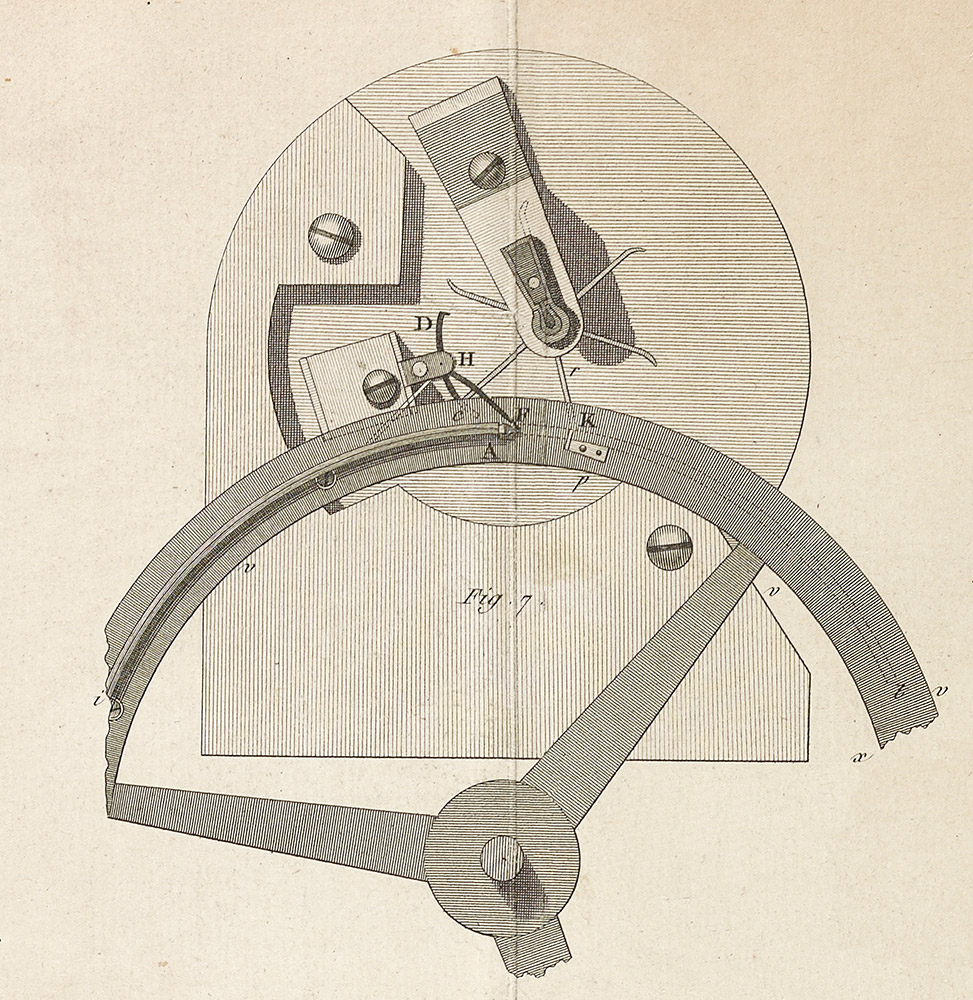
\includegraphics[scale=0.15]{Images/Le_Roy_escapement_mechanism}
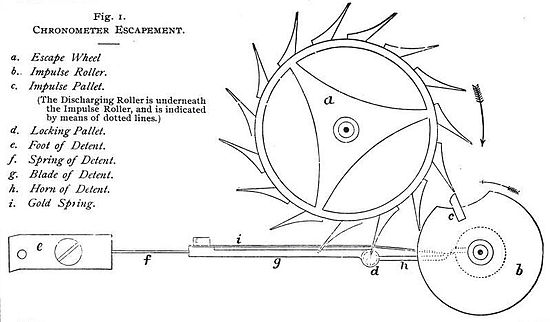
\includegraphics[scale=0.25]{Images/chronometer_detent_escapement}
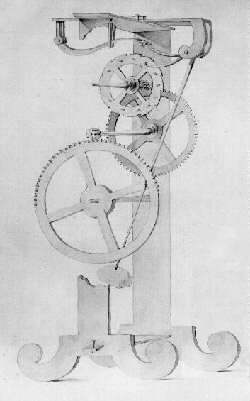
\includegraphics[scale=0.35]{Images/Galileo_Pendulum_Clock}
\end{frame}


\begin{frame}{Lesson 1}{}
{\Large\textbf{{The Analytical Engine}}}
\Large
\begin{minipage}{0.64\textwidth}
    \begin{itemize}
      \item The very first mechanical general purpose computer system
      \item Designed in 1837 by the English mathematician and computer pioneer Charles Babbage
      \item Built as a programmable device to solve different things  
    \end{itemize}
  \end{minipage}
\begin{minipage}{0.25\textwidth}
    % Show the image at item three and afterwards
      \begin{figure}
        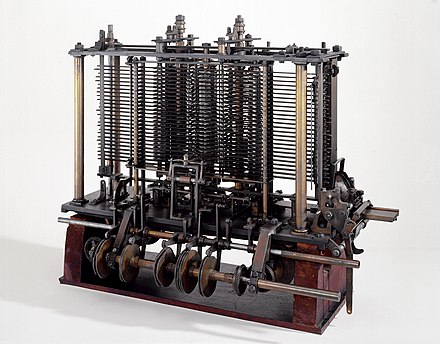
\includegraphics[scale=0.45]{Images/Babbages_AnalyticalEngine}
      \end{figure}
  \end{minipage}  
\end{frame}


\begin{frame}{Lesson 1}{}
{\Large\textbf{{Turing Machine}}}\\~\\
\begin{minipage}{0.57\textwidth}
\includegraphics[scale=0.24]{Images/Turing_Machine}
\end{minipage}
\Large
\begin{minipage}{0.42\textwidth}
    \begin{itemize}
      \item Infinite tape, divided into cells with symbols
      \item A head can read/write symbols on the tape
      \item A register that stores the state of the machine
    \end{itemize}
  \end{minipage}
\end{frame}



\begin{frame}{Lesson 1}{}
{\Large\textbf{{Modern calculator}}}
\Large
\begin{minipage}{0.70\textwidth}
    \begin{itemize}
      \item Execute a number of precise operations
      \item Designed to contain a set of such operations and instructions
      \item Includes even more complex operations, graphing charting
      \item Example: Texas Instruments
    \end{itemize}
  \end{minipage}
\begin{minipage}{.0\textwidth}
    % Show the image at item three and afterwards
      \begin{figure}
        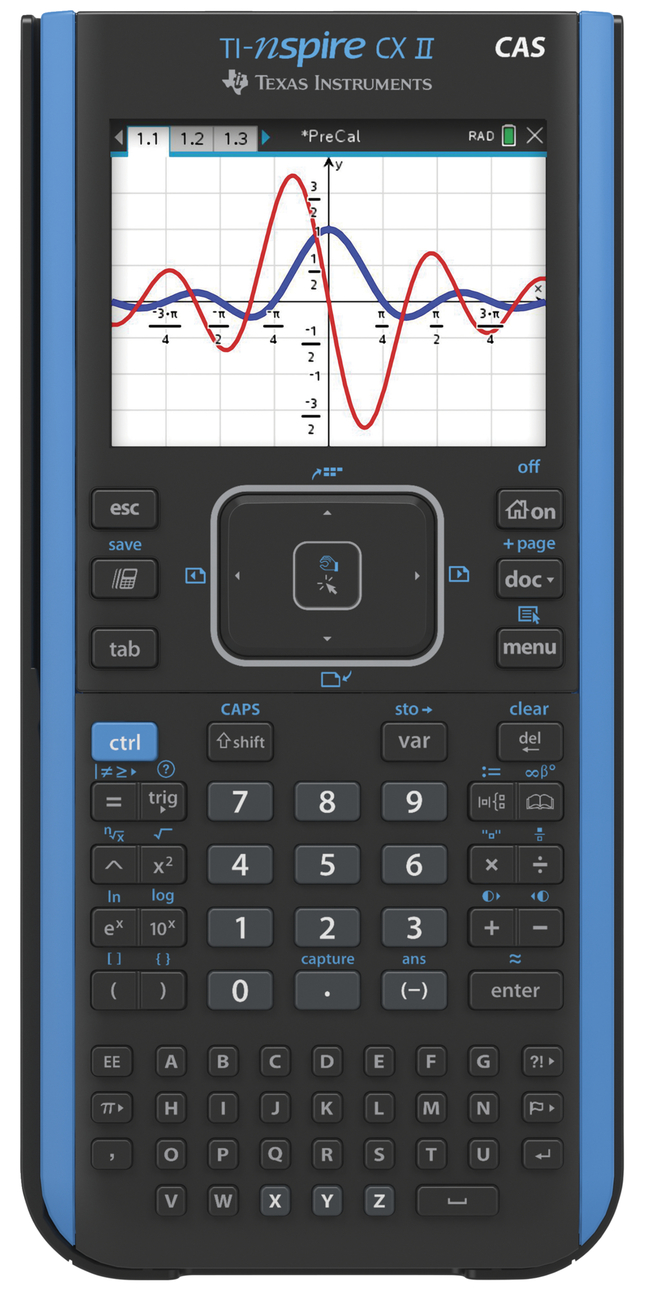
\includegraphics[scale=0.60]{Images/TI}
      \end{figure}
  \end{minipage}  
\end{frame}



\begin{frame}{Lesson 1}{}
{\Large\textbf{{Single-Board Computers (SBC)}}}
\Large
\begin{minipage}{0.65\textwidth}
    \begin{itemize}
      \item A simple computing device 
      \item CPU, GPU and Memory on a single chip
      \item Designed to run few applications
      \item Example: Raspberry PI 
    \end{itemize}
  \end{minipage}
\begin{minipage}{.0\textwidth}
    % Show the image at item three and afterwards
      \begin{figure}
        \includegraphics[scale=0.30]{Images/rbpi}
      \end{figure}
  \end{minipage}  
\end{frame}





\begin{frame}{Lesson 1}{}
{\Large\textbf{{Datacenter Servers}}}\\~\\
\begin{minipage}{0.50\textwidth}
\includegraphics[scale=0.38]{Images/sunfire}
\end{minipage}
\Large
\begin{minipage}{0.48\textwidth}
    \begin{itemize}
      \item Runs 24x7
      \item Enterprise applications
      \item Suitable for large number of users and applications 
      \item Available for data-centers
    \end{itemize}
  \end{minipage}
\end{frame}



\begin{frame}{Lesson 1}{}
\LARGE
Computation can be seen as a \textbf{sequence of states} a computing device does.\\~\\
\begin{itemize}
    \item Contains one or many sequence of states
    \item Can be an infinite number of sequence of states
    \item Or it can terminate with a final state
 \end{itemize}
\end{frame}



% --------------------------------------------------------------
% Algorithms 
% --------------------------------------------------------------
\begin{frame}{Lesson 1}{}
\begin{center}
\Huge Algorithms
\end{center}
\end{frame}

% What is an algorithm?
\begin{frame}{Lesson 1}{}
{\Huge{What is an algorithm?}}
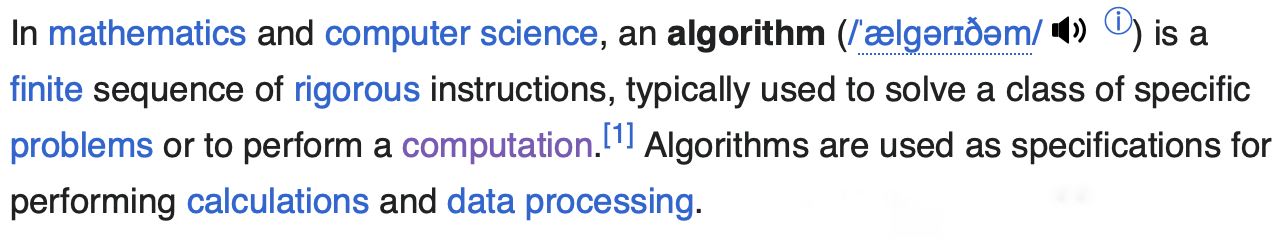
\includegraphics[scale=0.33]{Images/algorithm.png}

\Large{
\begin{itemize}
    \item But can we call this a \alert{computer program}?
    \item Or is it just a recipe, something higher than a \alert{sequence of code}
    \item A higher level of abstraction of how to implement something we plan to develop. Example: how to find a name in a phone book
\end{itemize}}

\end{frame}



\begin{frame}{Lesson 1}{}
\LARGE
\textbf{What is an algorithm?}\\~\\

\begin{center}

\tikzset{every picture/.style={line width=0.75pt}} %set default line width to 0.75pt        

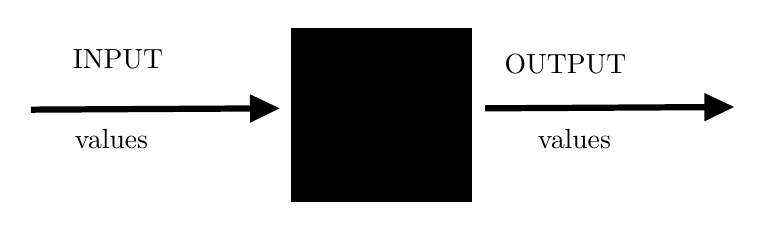
\begin{tikzpicture}[x=0.75pt,y=0.75pt,yscale=-1,xscale=1]
%uncomment if require: \path (0,171); %set diagram left start at 0, and has height of 171

%Shape: Rectangle [id:dp3842912892539916] 
\draw  [fill={rgb, 255:red, 0; green, 0; blue, 0 }  ,fill opacity=1 ][line width=2.25]  (349,57) -- (433,57) -- (433,138) -- (349,138) -- cycle ;
%Straight Lines [id:da6734653265949071] 
\draw [line width=2.25]    (440.9,94.36) -- (555.8,93.74) ;
\draw [shift={(560.8,93.71)}, rotate = 179.69] [fill={rgb, 255:red, 0; green, 0; blue, 0 }  ][line width=0.08]  [draw opacity=0] (14.29,-6.86) -- (0,0) -- (14.29,6.86) -- cycle    ;
%Straight Lines [id:da6306489033059055] 
\draw [line width=2.25]    (222,95) -- (336.9,94.38) ;
\draw [shift={(341.9,94.36)}, rotate = 179.69] [fill={rgb, 255:red, 0; green, 0; blue, 0 }  ][line width=0.08]  [draw opacity=0] (14.29,-6.86) -- (0,0) -- (14.29,6.86) -- cycle    ;


% Text Node
\draw (241,65) node [anchor=north west][inner sep=0.75pt]   [align=left] {INPUT};
% Text Node
\draw (242,103) node [anchor=north west][inner sep=0.75pt]   [align=left] {values};
% Text Node
\draw (449,67) node [anchor=north west][inner sep=0.75pt]   [align=left] {OUTPUT};
% Text Node
\draw (465,103) node [anchor=north west][inner sep=0.75pt]   [align=left] {values};

\end{tikzpicture}

$\overbrace{\hbox{Executes in a finite time}}^{\hbox{}}$

\end{center}

Sequence of computational steps that transform the input into the output

\end{frame}


\begin{frame}{Lesson 1}{Algorithms}
\Large
\textbf{Algorithms are everywhere}\\~\\ 
From your kitchen, in your microwave oven, your washing machine, to your phone or computer. When you browse Internet web sites your web browser is using different algorithms to decide how to display data to you.\\~\\
Our society relies on algorithms to suggest sentences for convicted criminals. You even use algorithms to keep you alive: the control systems from your car, or in different medical devices.
\end{frame}


\begin{frame}{Lesson 1}{Algorithms}
\Large
\textbf{But how can we describe them?}\\~\\ 
As an abstraction of something you plan to build or use, including all basic operations to achieve that. For example, think you plan to search in a phone book, a person phone number by the name:
\begin{itemize}
    \item you can start page by page searching for that name
    \item or you can jump directly to certain letters and start following from there
    \item or you can apply a different strategy, by 'cutting' the book into half, checking the letter in which half belongs, and applying all over again the same principle until the name is found
\end{itemize}
\end{frame}


\begin{frame}{Lesson 1}{Algorithms}
\Large
\textbf{How can we write one algorithm?}\\~\\ 
You can write it in plain English or in a more precise way using mathematics. Some others are using a form of \alert{pseudocode}.\\~\\
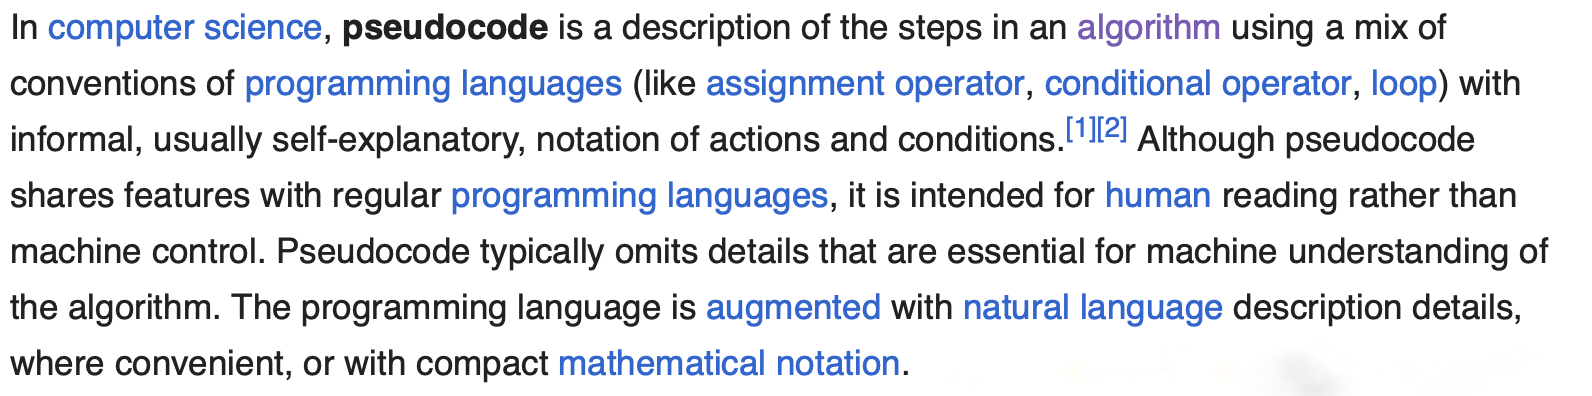
\includegraphics[scale=0.27]{Images/pseudocode}

\end{frame}



\begin{frame}{Lesson 1}{Algorithms}
\Large
\textbf{Example phonebook}\\~\\

\label{phonebook}

\begin{algorithmic}[1]

\Procedure{PhoneBook}{$N$}\Comment{Returns person name: N}
\State $N\gets 1$
\State Open page number $N$
\State Look at the page $N$
\If {Person is on page $N$}
    \State \textbf{Call person} $N$\Comment{The person name is $N$}
\Else \State \textbf{Find next page.} {$N\gets $N + 1} Go back to 3 
\EndIf
\EndProcedure
\end{algorithmic}
\end{frame}


\begin{frame}
\begin{center}
\Huge 
\textbf {Can we write an algorithm as a diagram?}
\end{center}
\end{frame}

\begin{frame}{Lesson 1}{}
\LARGE
\textbf{Flowcharts}
\end{frame}


\begin{frame}{Lesson 1}{}
{\Large\textbf{{Algorithms as flowcharts. What is a flowchart?}}} 
\Large
\begin{minipage}{0.60\textwidth}
    \begin{itemize}
	  \item is a type of technical diagram
      \item that represents a workflow or a process
      \item a sequence of states
      \item including their specific order
    \end{itemize}
  \end{minipage}
\begin{minipage}{.\textwidth}
    % Show the image at item three and afterwards
      \begin{figure}
        \includegraphics[scale=0.19]{Images/flowchart11}
      \end{figure}
  \end{minipage}  
\end{frame}


\begin{frame}{Lesson 1}{}
\begin{center}
\includegraphics[scale=0.15]{Images/flowchart2}
\end{center}
\end{frame}


% What is an algorithm?
\begin{frame}{Lesson 1}{Algorithm}
{\Large\textbf{{What is a flowchart?}}}
\includegraphics[scale=0.45]{Images/flowchart-info.png}
\end{frame}



\begin{frame}{Lesson 1}{}
\LARGE
\textbf{Flowchart diagram}\\~\\
\begin{itemize}
	\item describes the sequence of movements or actions of people or things involved in a complex system or activity
	\item a graphical representation of a computer program in relation to its sequence of functions (distinct from the data it processes).
\end{itemize}
\end{frame}


\begin{frame}
\begin{center}
\Huge 
\textbf {Yes, we can write and define an algorithm as a flowchart}
\end{center}
\end{frame}


\begin{frame}{Lesson 1}{}
\LARGE
\textbf{Functional block diagrams}
\end{frame}


% What is an algorithm?
\begin{frame}{Lesson 1}{Algorithm}
\includegraphics[scale=0.60]{Images/fbd.png}
\end{frame}


\begin{frame}{Lesson 1}{}
\LARGE
\textbf{The functional block diagram}\\~\\
Another type of diagram, a specialized high-level type of flow chart.\\~\\
\textbf {We can specify and describe the modules of a complex system}
\end{frame}


\begin{frame}{Lesson 1}{}
\LARGE
\textbf{The functional block diagram}\\~\\
Functional block diagrams (FBD) describe system relationships along with their main functions. It is the basic, canonical document for any system or application before drawing any other more complex technical design plans. These diagrams are widely used in hardware engineering.
\end{frame}


\begin{frame}{Lesson 1}{}
\LARGE
\textbf{Functional block diagram}\\~\\
\begin{itemize}
	\item describes the relationships of a system, by specifying their main functions, including the input and output of each main modules and components
	\item the input and output elements of a block representing by lines
	\item the relationships between the functions or modules
	\item the functional sequences and paths for the data flow
\end{itemize}
\end{frame}


\begin{frame}{Lesson 1}{Algorithm}
\begin{center}
	\includegraphics[scale=1.30]{Images/fbd0}
\end{center}
\end{frame}


\begin{frame}{Lesson 1}{Algorithm}
\begin{center}
	\includegraphics[scale=0.30]{Images/fbd1}
\end{center}
\end{frame}


\begin{frame}{Lesson 1}{Algorithm}
\begin{center}
	\includegraphics[scale=0.28]{Images/fbd2}
\end{center}
\end{frame}


\begin{frame}
\begin{center}
\Huge 
\textbf {Functional block diagrams are better to describe and document entire systems, their components and data flows, not algorithms. Use a flowchart for that!}
\end{center}
\end{frame}


\begin{frame}{Lesson 1}{Algorithms}
\Large
\textbf{But why not using a programming language?}\\~\\ 
We must think what we are planning to do, and how we plan to do it. And for that, we must not rely on a programming language: we will be restricted by the limits of the specific programming language not being abe to design and think freely about it.\\~\\
A better approach is to think to write it as pseudocode or simple mathematics. This way we can have all flexibility and the power of precise mathematics.
\end{frame}


\begin{frame}{Lesson 1}{Algorithms}
\Large
\textbf{Euclid's Algorithm or GCD}\\~\\ 
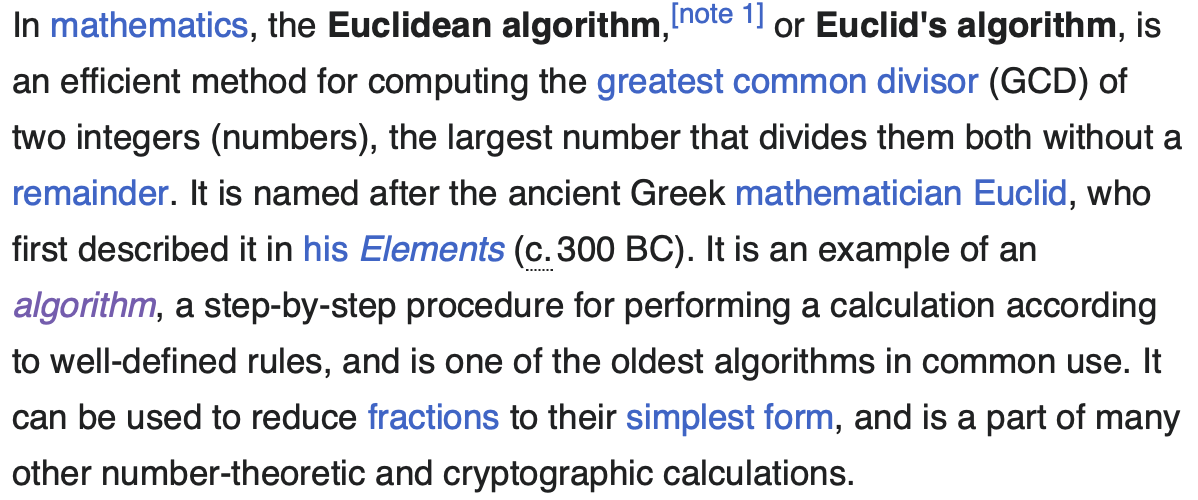
\includegraphics[scale=0.7]{Images/gcd}
\end{frame}

\begin{frame}{Lesson 1}{Algorithms}
\Large
\textbf{Euclid's Algorithm}\\~\\ 
Greatest Common Divisor (GCD) of two numbers A and B is the largest number that divides both A and B. (Number here defined as an \alert{integer})\\~\\

An integer is the number zero (0), a positive natural number (1, 2, 3, etc) or a negative integer with a minus sign (-1, -2, -3, etc) In mathematics we call this \(\mathbb{Z}\) set of numbers.
\end{frame}


\begin{frame}{Lesson 1}{Algorithms}
\Large
\textbf{Euclid's Algorithm}\\~\\
The very first version:\\~\\ 
If A = 0 then GCD(A,B)=B, since the GCD(0,B)=B, and STOP\\  
If B = 0 then GCD(A,B)=A, since the GCD(A,0)=A, and STOP\\  
Write A in quotient remainder form (A = B * Q + R)\\
Compute then GCD(B,R) since GCD(A,B) = GCD(B,R)
\end{frame}


\begin{frame}{Lesson 1}{Algorithms}
\Large
\textbf{Euclid's Algorithm, pseudocode}\\~\\

\label{GCD}
\begin{algorithmic}[1]
\Procedure{GCD}{$A,B$}\Comment{The g.c.d. of A and B}
   \State $R\gets A\bmod B$
   \While{$R\not=0$}\Comment{We have the answer if R is 0}
      \State $A\gets B$
      \State $B\gets r$
      \State $R\gets A\bmod B$
   \EndWhile\label{GCDendwhile}
   \State \textbf{return} $B$\Comment{The gcd is B}
\EndProcedure
\end{algorithmic}
\end{frame}



\begin{frame}{Lesson 1}{Algorithms}
\Large
\textbf{Euclid's Algorithm, improved}\\~\\

\label{Euclid}
\begin{algorithmic}[1]
\Procedure{Euclid}{$A,B$}\Comment{The g.c.d. of A and B}
\If{$B==0$}
    \State \textbf{return} $A$\Comment{The gcd is A}
\Else \State \textbf{return} \Call{Euclid}{$B, A\bmod B$}
\EndIf
\EndProcedure
\end{algorithmic}
\end{frame}



\begin{frame}{Lesson 1}{Algorithms}
\Large
\textbf{Euclid's Algorithm, using mathematics}\\~\\
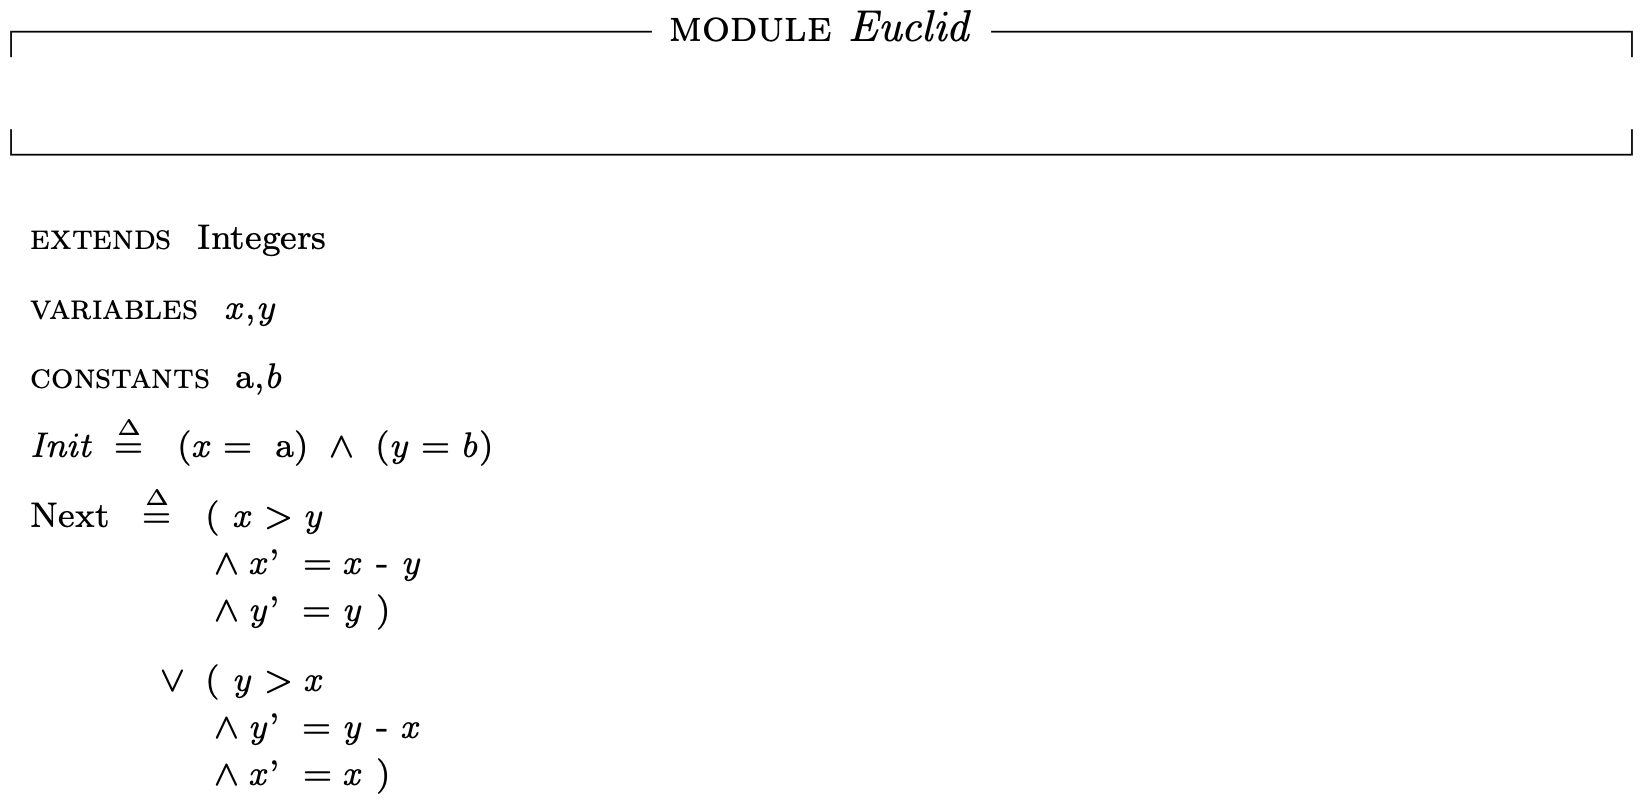
\includegraphics[scale=0.5]{Images/gcdtla}
\end{frame}


\begin{frame}
\begin{center}
\Huge 
\textbf {But how do we know our algorithm does the right thing?}
\end{center}
\end{frame}


\begin{frame}{Lesson 1}{}
\LARGE
\textbf {"An algorithm for a computational problem is CORRECT if, for every problem instance provided as input it HALTS, finishes its computing  in finite time and outputs the correct solution to the problem instance"\\~\\}
A correct algorithm SOLVES the given computational problem

\end{frame}



\begin{frame}{Lesson 1}{}
\LARGE
\textbf {An incorrect algorithm might not HALT at all on some input instances, or it might halt with an incorrect answer\\~\\}
\end{frame}



\begin{frame}{Lesson 1}{Algorithms}
\Large
\textbf{Classes of algorithms}\\~\\ 
    \begin{multicols}{3}
    \begin{itemize}
        \item Divide and Conquer
        \item Sorting
        \item Searching
        \item Dynamic programming
        \item Greedy algorithms
        \item Graph algorithms
        \item Shortest path
        \item Maximum flow
        \item Parallel algorithms
        \item Matrix operations
        \item Online algorithms
        \item Machine learning
        \item Linear programming
        \item String matching
    \end{itemize}
    \end{multicols}
\end{frame}


\begin{frame}
\begin{center}
\Huge 
\textbf { How about AI? }
\end{center}
\end{frame}


\begin{frame}{Lesson 1}{}
\LARGE
\textbf {Still an algorithm\\~\\}
\begin{itemize}
    \item Or more precisely many algorithms
    \item Complex algorithms
    \item But still algorithms nevertheless 
 \end{itemize}
\end{frame}


\begin{frame}{Lesson 1}{}
\includegraphics[scale=0.3]{Images/AI}
\end{frame}


\begin{frame}
\frametitle{Lesson 1}

\Huge Algorithms 
\alert{dont feel} are not 
 \alert{conscious},
 \alert{sentient beings}!
\end{frame}



\begin{frame}
\frametitle{Lesson 1}
\huge
\textbf {We need safe and secure software\\~\\}
\begin{itemize}
	 \item predictable - \alert{which we can CONTROL}
	 \item not harmful - \alert{USEFUL to us}
	 \item \alert{being able to STOP it if we want}
\end{itemize}
\end{frame}


\begin{frame}
\frametitle{Lesson 1}
\huge
\textbf {This is not about being nice, but rather being able to describe and proof that our algorithms do the right thing and do it efficiently based on mathematically tools\\~\\}

This is what we need.
\end{frame}




% --------------------------------------------------------------
% Programs 
% --------------------------------------------------------------
\begin{frame}{Lesson 1}{}
\begin{center}
\Huge Computer Programs
\end{center}
\end{frame}


% What is a computer program?
% What is an algorithm?
\begin{frame}{Lesson 1}{}
{\Huge{What is a computer program?}}
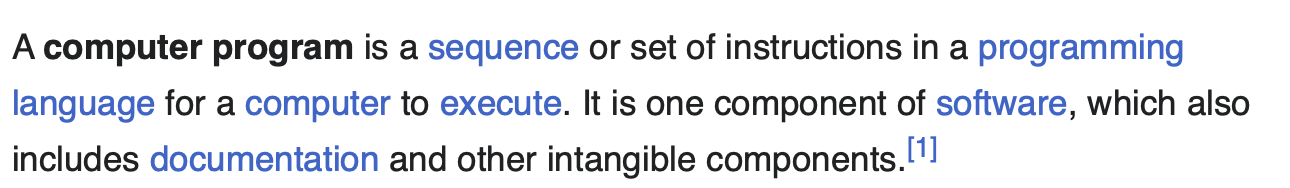
\includegraphics[scale=0.67]{Images/program}
\end{frame}


\begin{frame}{Lesson 1}{}
\Large
\textbf{How to think about programs}\\~\\

\Large{
\begin{itemize}
    \item We should think like engineers or computer scientists
    \item Scientific thinking is very successful
    \item Science makes mathematical models of reality
	\item Digital systems, processors, storage devices
    \item We model how computers are executing programs
\end{itemize}}

\end{frame}



\begin{frame}{Lesson 1}{}
\Large
\textbf{Basic models}\\~\\

\Large{
\begin{itemize}
    \item Touring machines 
    \item Functions
    \item Automata
    \item Sequence of states
\end{itemize}}

\end{frame}




\begin{frame}{Lesson 1}{}
\Large
\textbf{Program. Computation. Sequence of States}\\~\\

\Large{
\begin{itemize}
    \item A program execution is a computation (behaviour)
    \item A computation is a sequence of states    
    \item A state is an assignment of values to variables
\end{itemize}}

\Large {A program is modeled as a set of computations, representing all possible program executions}
\end{frame}




%\begin{frame}{Lesson 1}{}

%{\Huge{Alogrithm or Program? Is a program an algorithm?}}

%\Large
%\textbf{An algorithm is an abstract program?}\\~\\
%\end{frame}


\begin{frame}{Lesson 1}{}
\Huge Computers, digital systems are executing programs
\end{frame}


\begin{frame}{Lesson 1}{}
\Large
\textbf{From source code to executable}\\~\\ 
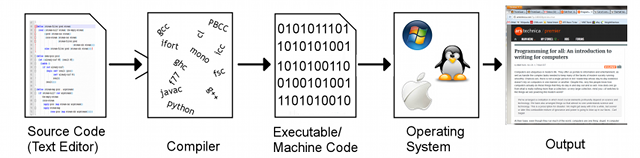
\includegraphics[scale=0.65]{Images/CompilationChain}
\end{frame}


\begin{frame}{Lesson 1}{}
{\Huge{Program structure}}
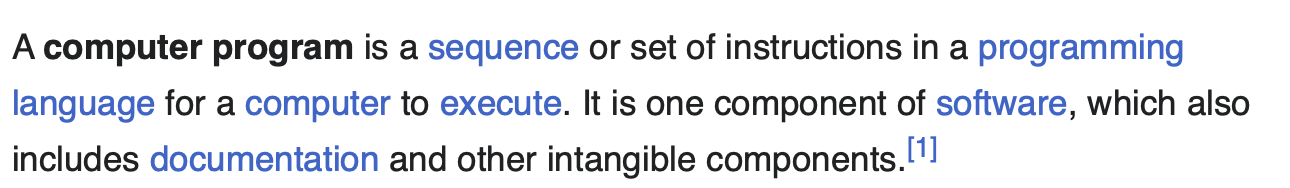
\includegraphics[scale=0.67]{Images/program}

\Large{
\begin{itemize}
    \item Some programs run forever, some dont
    \item A program execution is defined by at least one computation
    \item A computation is a sequence of states
    \item And a state is an assignment of values to variables
\end{itemize}}

\end{frame}


\begin{frame}{Lesson 1}{}
{\Huge{Program types}}\\~\\ 

\Large{
\begin{itemize}
    \item A program is modelled by a set of computations, representing all possible executions
    \item Remember an algorithm is just an abstract program
    \item Different programs: software applications and system software
    \item System software: operating systems
\end{itemize}}
\end{frame}


\begin{frame}{Lesson 1}{}
{\Large\textbf{{Application and System Programs}}}

\Large
\begin{minipage}{0.65\textwidth}
    \begin{itemize}
      \item \textbf{Software applications}:  enterprise resource planning, customer relationship management, supply chain management software, web, middleware, databases
      \item \textbf{Operating systems}: macOS, RedHat, FreeBSD, Windows
    \end{itemize}
  \end{minipage}
\begin{minipage}{0.30\textwidth}
    % Show the image at item three and afterwards
      \begin{figure}
        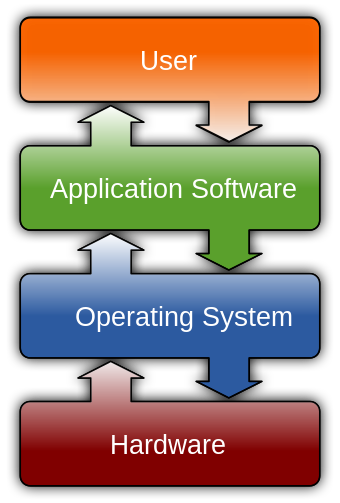
\includegraphics[scale=0.32]{Images/OS}
      \end{figure}
  \end{minipage}
\end{frame}


\begin{frame}{Lesson 1}{Programs}
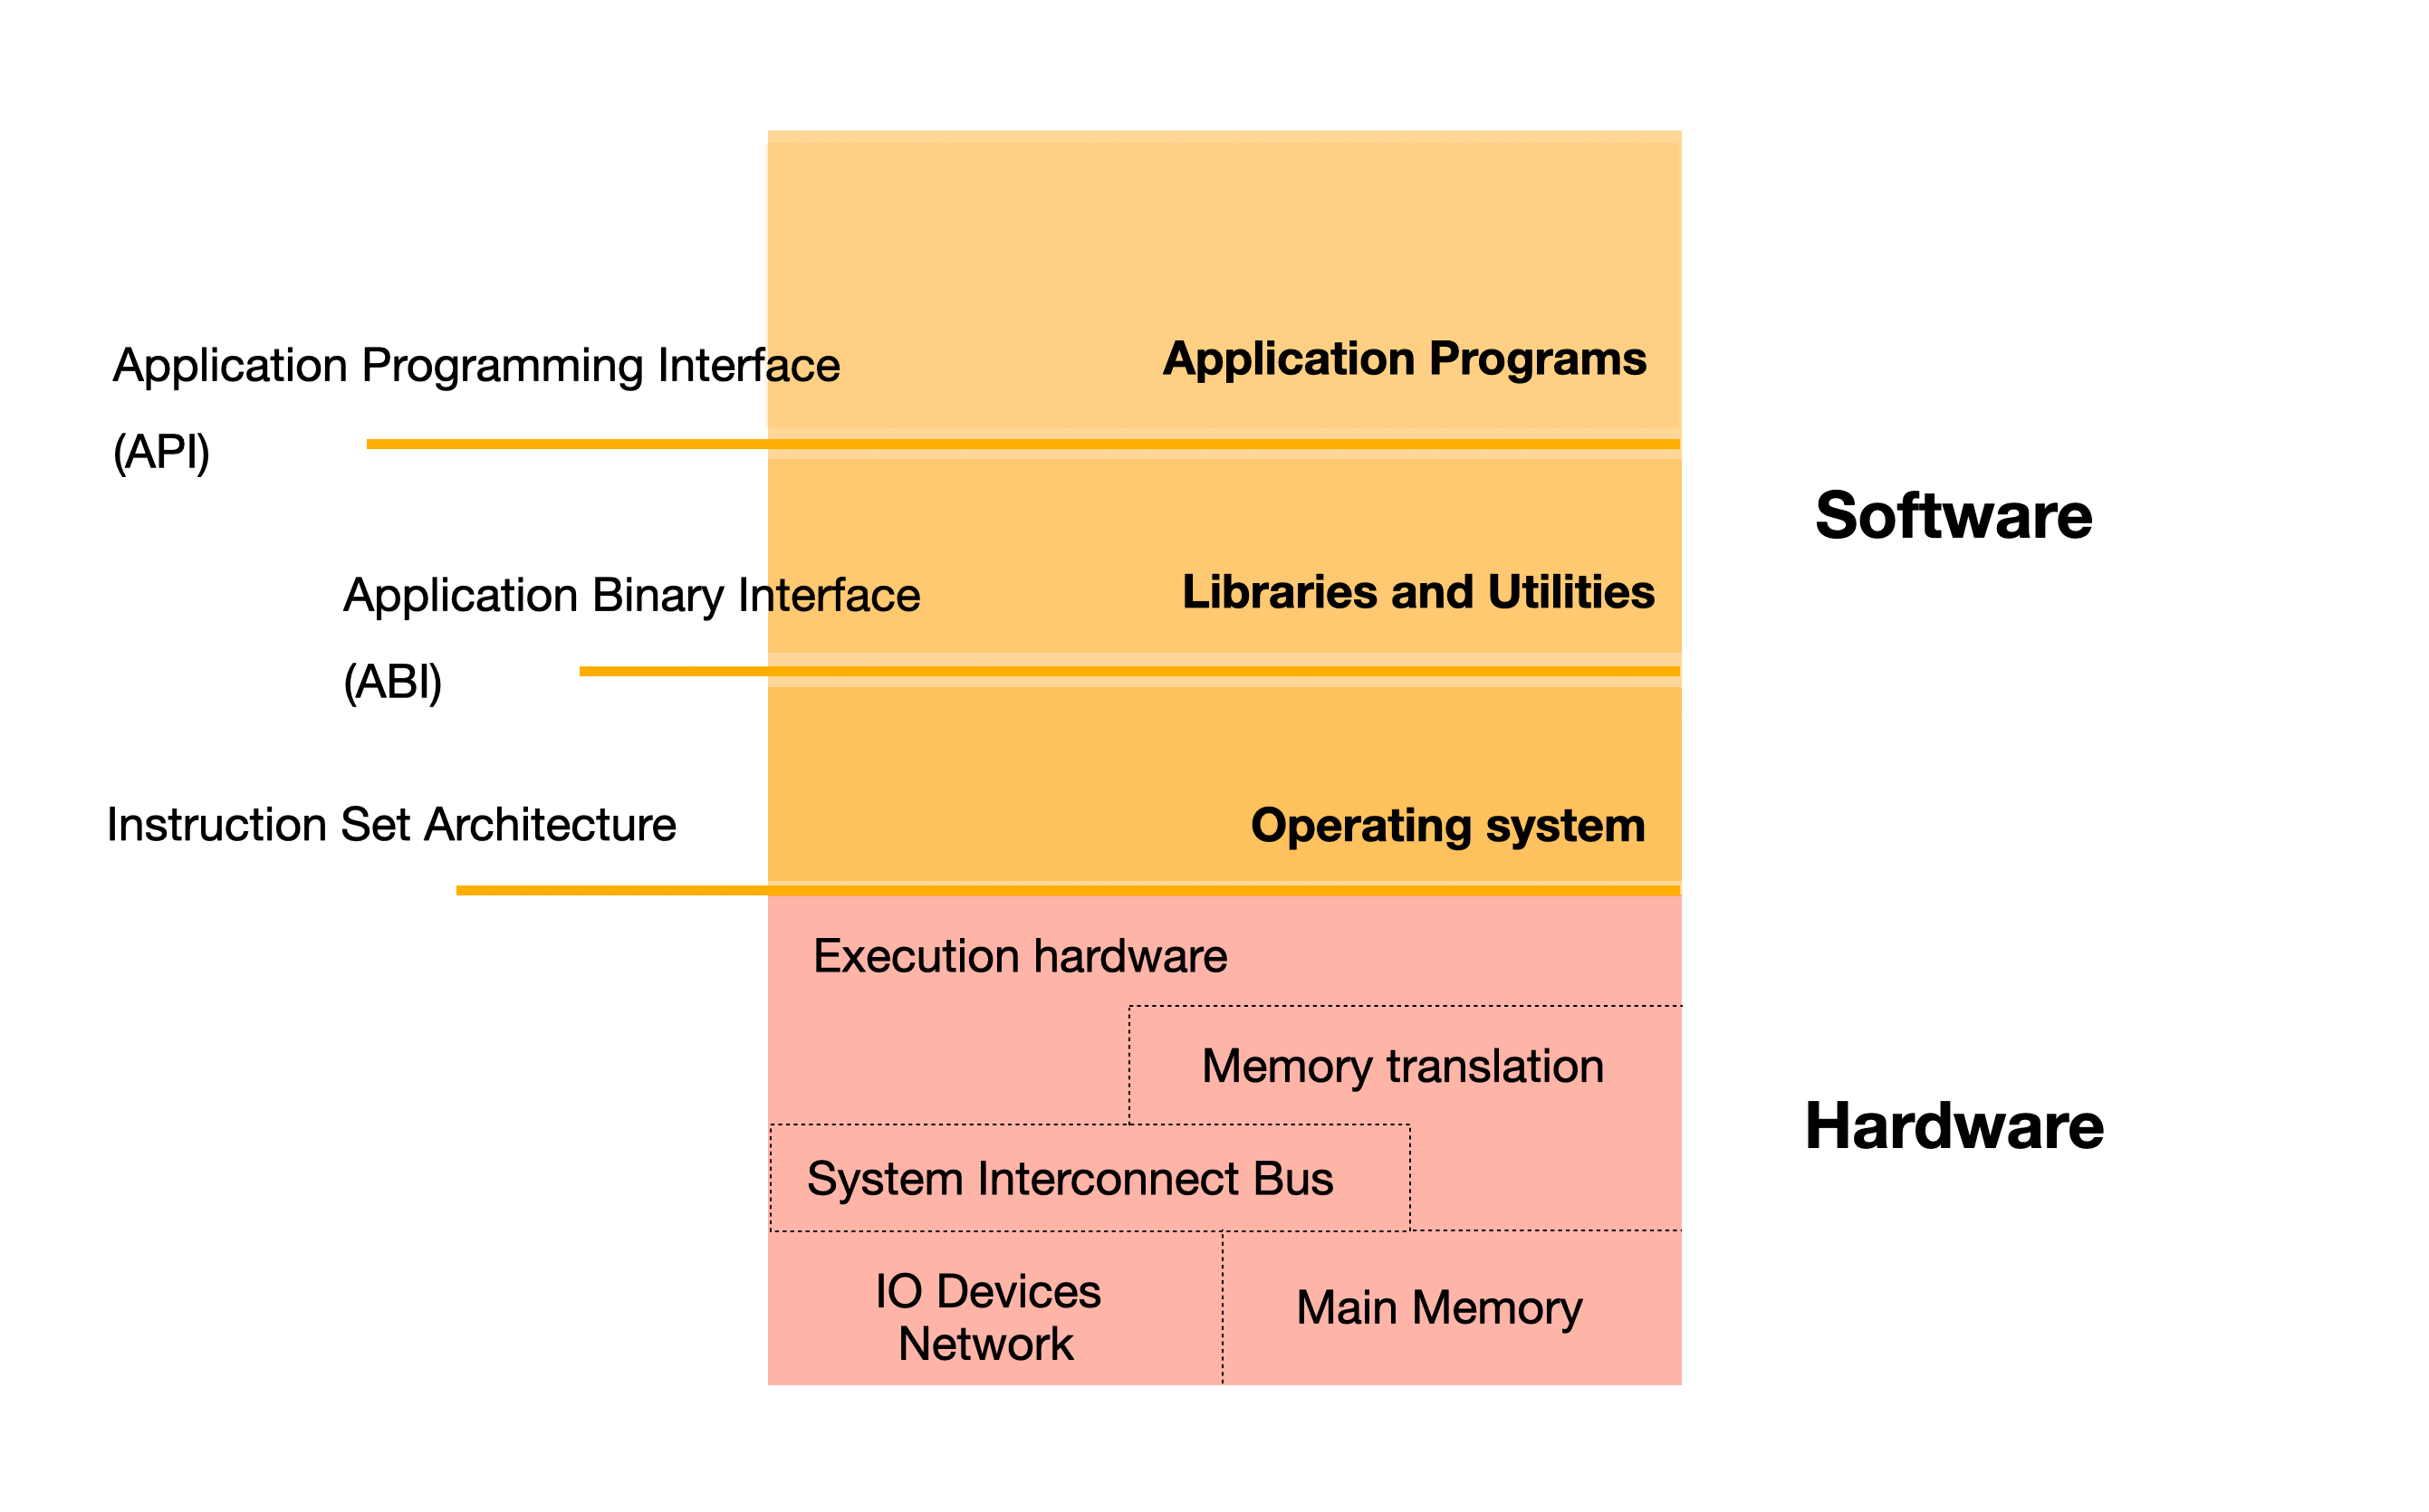
\includegraphics[scale=0.15]{Images/sfwhdw}
\end{frame}





%\begin{frame}
%\frametitle{Lesson 1}

%\Large{Computation}
%In this slide, some important text will be
%\alert{highlighted} because it's important.
%Please, don't abuse it.

%\begin{block}{Remark}
%Sample text
%\end{block}

%\begin{alertblock}{Important theorem}
%Sample text in red box
%\end{alertblock}

%\begin{examples}
%Sample text in green box. The title of the block is ``Examples".
%\end{examples}
%\end{frame}



% -------------------------------------------------------------------
% Lesson 2
% -------------------------------------------------------------------
\section{Software specifications. Formal methods}

\begin{frame}
\begin{center}
\Huge Lesson 2\\
Software speifications. Formal methods
\end{center}
\end{frame}



%\begin{frame}{What is programming?}{Coding is the easy part of programming}

%\Large{
%Programming is not coding. Is more than that. We must think WHAT and HOW to write and implement a program BEFORE starting any coding!
%Programming consists of the following actions:}

%\begin{description}
%    \item[WHAT] We need to think what the program should do. If you dont think carefully enough about that you will have a program not operating correctly.
    
%    \item[HOW] Deciding how the program should be implemented. Thats should be at the algorithm level, rather than code level. Think how the problem should be implemented, above the code level.
    
%    \item[DO IT] Start coding, using a specific programming language, like Java, Rust, Python
%\end{description}
%\end{frame}


%\begin{frame}{Blocks in beamer}{}
%\begin{block}{Block 1}
%This is a simple block in beamer.
%\end{block}
%\end{frame}


%\begin{frame}
%\frametitle{Two-column slide}
%\begin{columns}
%\column{0.5\textwidth}
%This is a text in first column.
%$$E=mc^2$$
%\begin{itemize}
%\item First item
%\item Second item
%\end{itemize}

%\column{0.5\textwidth}
%This text will be in the second column
%and on a second thoughts, this is a nice looking
%layout in some cases.
%\end{columns}
%\end{frame}



% -------------------------------------------------------------------
% Lesson 3
% -------------------------------------------------------------------
\section{Data Structures and Algorithms }

\begin{frame}
\begin{center}
\Huge Lesson 3\\
Data Structures and Algorithms
\end{center}
\end{frame}




% -------------------------------------------------------------------
% Lesson 4
% -------------------------------------------------------------------
\section{Programming vs Coding}

\begin{frame}
\begin{center}
\Huge Lesson 4\\
Programming vs Coding
\end{center}
\end{frame}


% -------------------------------------------------------------------
% Lesson 5
% -------------------------------------------------------------------
\section{Data Ingestion, Transformation, Analysis}

\begin{frame}
\begin{center}
\Huge Lesson 5\\
Data Capturing, Transformation, Analysis
\end{center}
\end{frame}



% -------------------------------------------------------------------
% Lesson 6
% -------------------------------------------------------------------
\section{Build Safe and Secure Software}
\begin{frame}
\begin{center}
\Huge Lesson 6\\
Build Safe and Secure Software
\end{center}
\end{frame}


% -------------------------------------------------------------------
% Lesson 7
% -------------------------------------------------------------------
\section{System Performance Analysis}
\begin{frame}
\begin{center}
\Huge Lesson 7\\
System Performance Analysis
\end{center}
\end{frame}


\end{document}

